\documentclass[10pt,a4paper]{article}
\usepackage[utf8]{inputenc}
\usepackage[T1]{fontenc}
\usepackage{amsmath}
\usepackage{amssymb}
\usepackage{graphicx}
\usepackage{hyperref}
\usepackage{float}
\usepackage{subcaption}
\usepackage{geometry}
\geometry{a4paper, margin=1in}

\title{Exploring the Platonic Representation Hypothesis Beyond In-Distribution Data}
\author{Aryasomayajula Ram Bharadwaj\\
Independent Researcher\\
\texttt{ram.bharadwaj.arya@gmail.com}}
\date{20th Oct 2024}

\begin{document}

\maketitle

\begin{abstract}
The Platonic Representation Hypothesis (PRH) \cite{huh2024prh} posits that neural networks, despite being trained on different objectives and datasets, converge toward a shared statistical model of reality. This paper extends the investigation of PRH to out-of-distribution (OOD) settings, using ImageNet-O as a benchmark, and contrasts the findings with results from in-distribution data, random noise, and the dynamics of model alignment under noise injection and during language model training. Our analysis reveals that while PRH holds in OOD scenarios, it breaks down with purely random data, and demonstrates a nuanced relationship between noise and representational alignment.
\end{abstract}

\section{Introduction}
The PRH suggests that models trained across various modalities and objectives converge toward a shared representation of reality \cite{huh2024prh}. Inspired by philosophical concepts like Plato’s Allegory of the Cave, PRH proposes that neural networks are progressively learning an idealized representation of the world. This convergence has been observed across domains such as vision and language models, with evidence showing that larger models better align their internal representations \cite{huh2024prh}. However, it remains unclear whether such convergence persists when models encounter data significantly different from their training distribution.

To address this, we extend PRH's analysis to out-of-distribution (OOD) settings using the ImageNet-O dataset, which contains samples outside the distribution of ImageNet \cite{hendrycks2021nae}. We also include random noise as a contrasting dataset to examine the boundaries of representational alignment, along with two additional experiments: the impact of progressive noise on alignment among vision models and the evolution of alignment during language model training.

\section{Methodology}
We assess representational alignment using various metrics, such as mutual k-NN and CKNN-A, across three types of data:
\begin{enumerate}
    \item \textbf{In-distribution data}: Data that aligns with the pretraining dataset (e.g., Places365’s validation set).
    \item \textbf{Out-of-distribution data}: ImageNet-O, designed with images that are outliers to the ImageNet distribution \cite{hendrycks2021nae}.
    \item \textbf{Random noise}: Purely random images to test the limits of PRH.
\end{enumerate}
The alignment between different models is measured using Spearman's rank correlation, focusing on how similar the models' distance measures are for given data points. Throughout the experiments, 17 different Vision Transformers spanning different sizes and trained data are used. Mutual k-Nearest Neighbor Alignment is measured in all the three settings.

We also conducted two additional analyses:
\begin{enumerate}
    \item \textbf{Noise Injection in Vision Models}: A set of 250 images was progressively corrupted with noise in 100 steps, and mutual alignment was measured across all pairs of the 17 ViT models at each step. The mean alignment scores were analyzed to study the relationship between noise levels and model alignment.
    \item \textbf{Training Dynamics in Language Models}: Six large language models (LLMs) were analyzed using checkpoints saved at 100 different training stages. We measured the alignment of each model pair at each stage and examined the trends in alignment throughout the training process.
\end{enumerate}

\section{Results}

\subsection{Alignment on In-Distribution Data}
\begin{figure}[H]
    \centering
    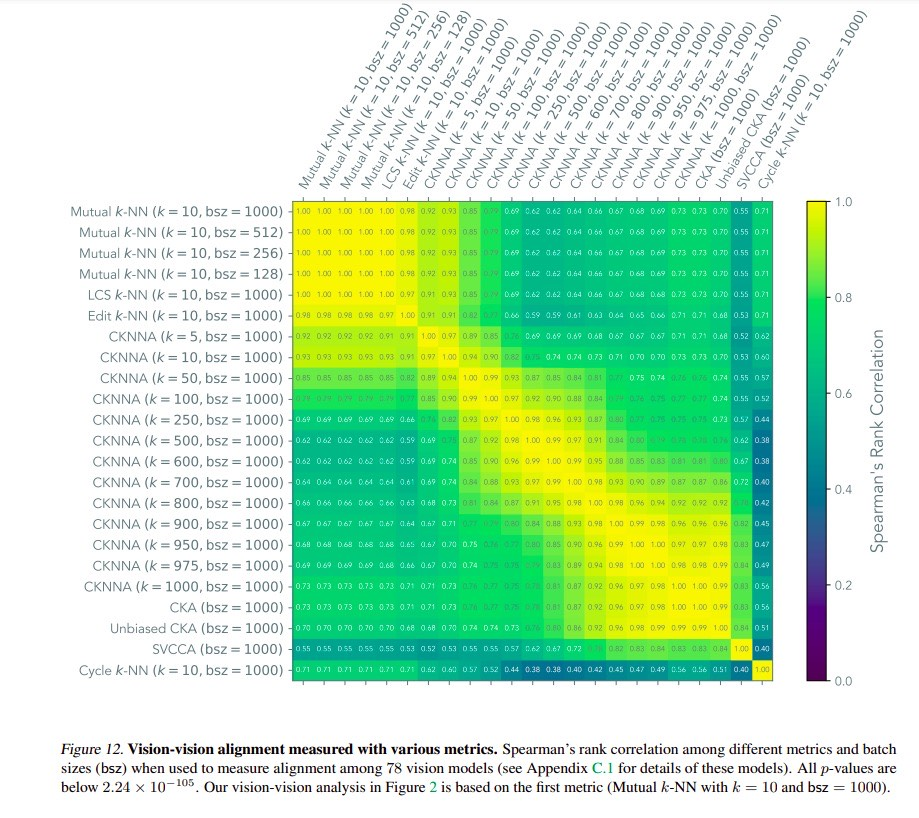
\includegraphics[width=\textwidth]{prh_correlation.jpg}
    \caption{Vision-vision alignment measured on Places365’s validation dataset using various metrics. High Spearman's rank correlation among different metrics indicates alignment among vision models.}
    \label{fig:prh_correlation}
\end{figure}

\subsection{Alignment on ImageNet-O}
\begin{figure}[H]
    \centering
    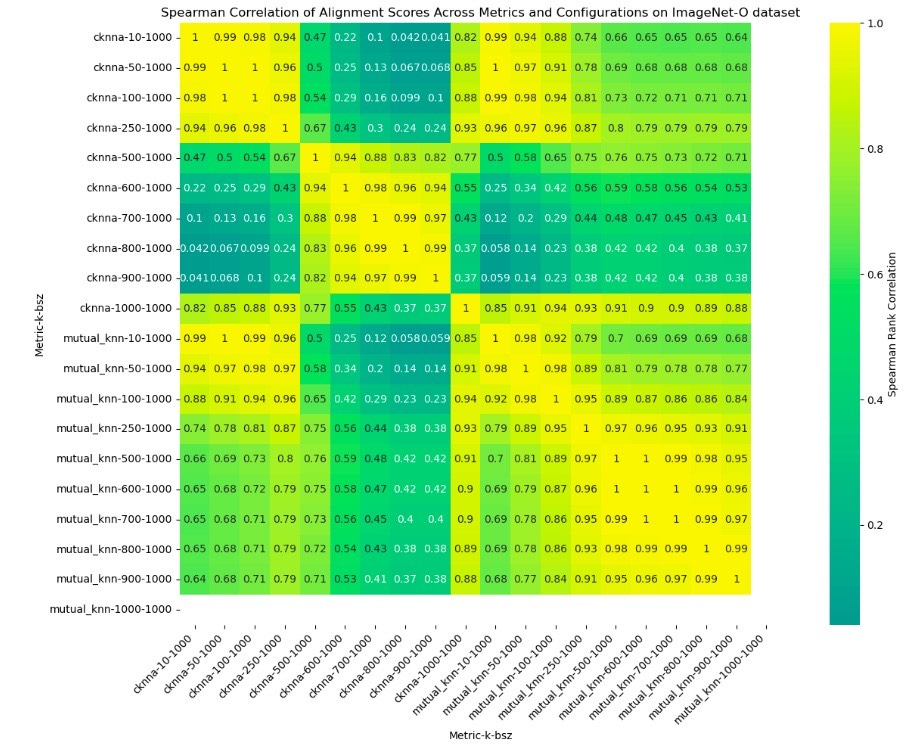
\includegraphics[width=\textwidth]{prh_correlation_ood.jpg}
    \caption{Alignment of vision models on ImageNet-O dataset. The Spearman correlation suggests that even with outlier data, models maintain a shared statistical representation, albeit with higher prediction errors.}
    \label{fig:prh_correlation_ood}
\end{figure}

\subsection{Alignment on Random Data}
\begin{figure}[H]
    \centering
    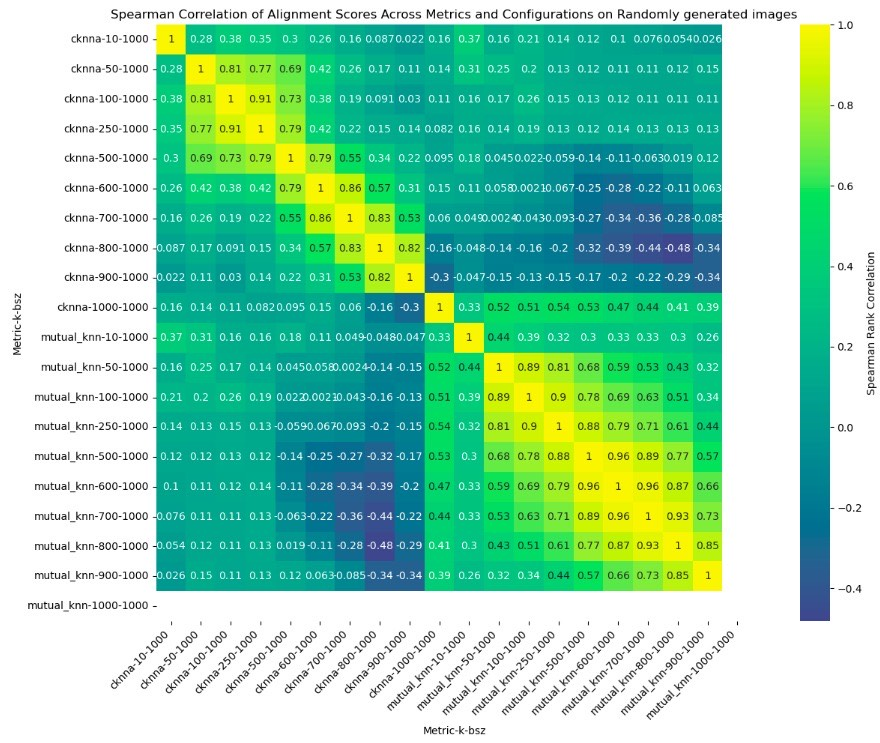
\includegraphics[width=\textwidth]{prh_correlation_random.jpg}
    \caption{Spearman correlation of alignment scores on random noise data. The lower correlation values indicate a breakdown in representational alignment, suggesting that random data lacks the underlying structure needed for PRH.}
    \label{fig:prh_correlation_random}
\end{figure}

\subsection{Noise Injection in Vision Models}
\begin{figure}[H]
    \centering
    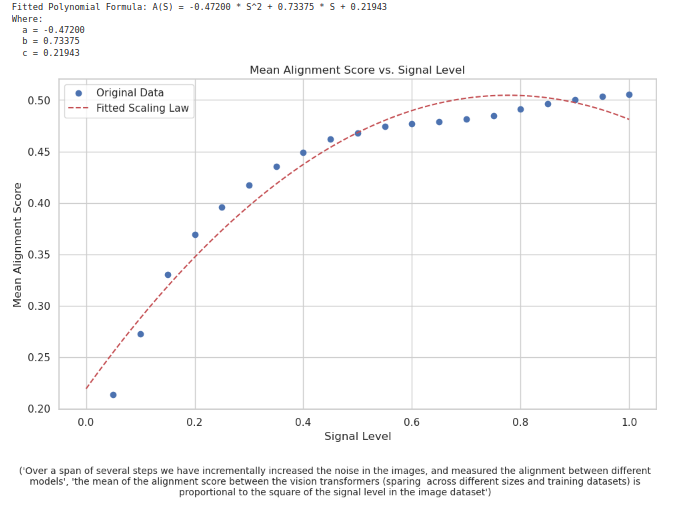
\includegraphics[width=\textwidth]{alignment_vs_signal_level.png}
    \caption{Mean alignment of 17 ViT models with respect to signal level (1 - noise) across 100 noise injection steps. The alignment shows a quadratic relationship with decreasing signal levels.}
    \label{fig:alignment_vs_signal_level}
\end{figure}

\subsection{Training Dynamics in Language Models}
\begin{figure}[H]
    \centering
    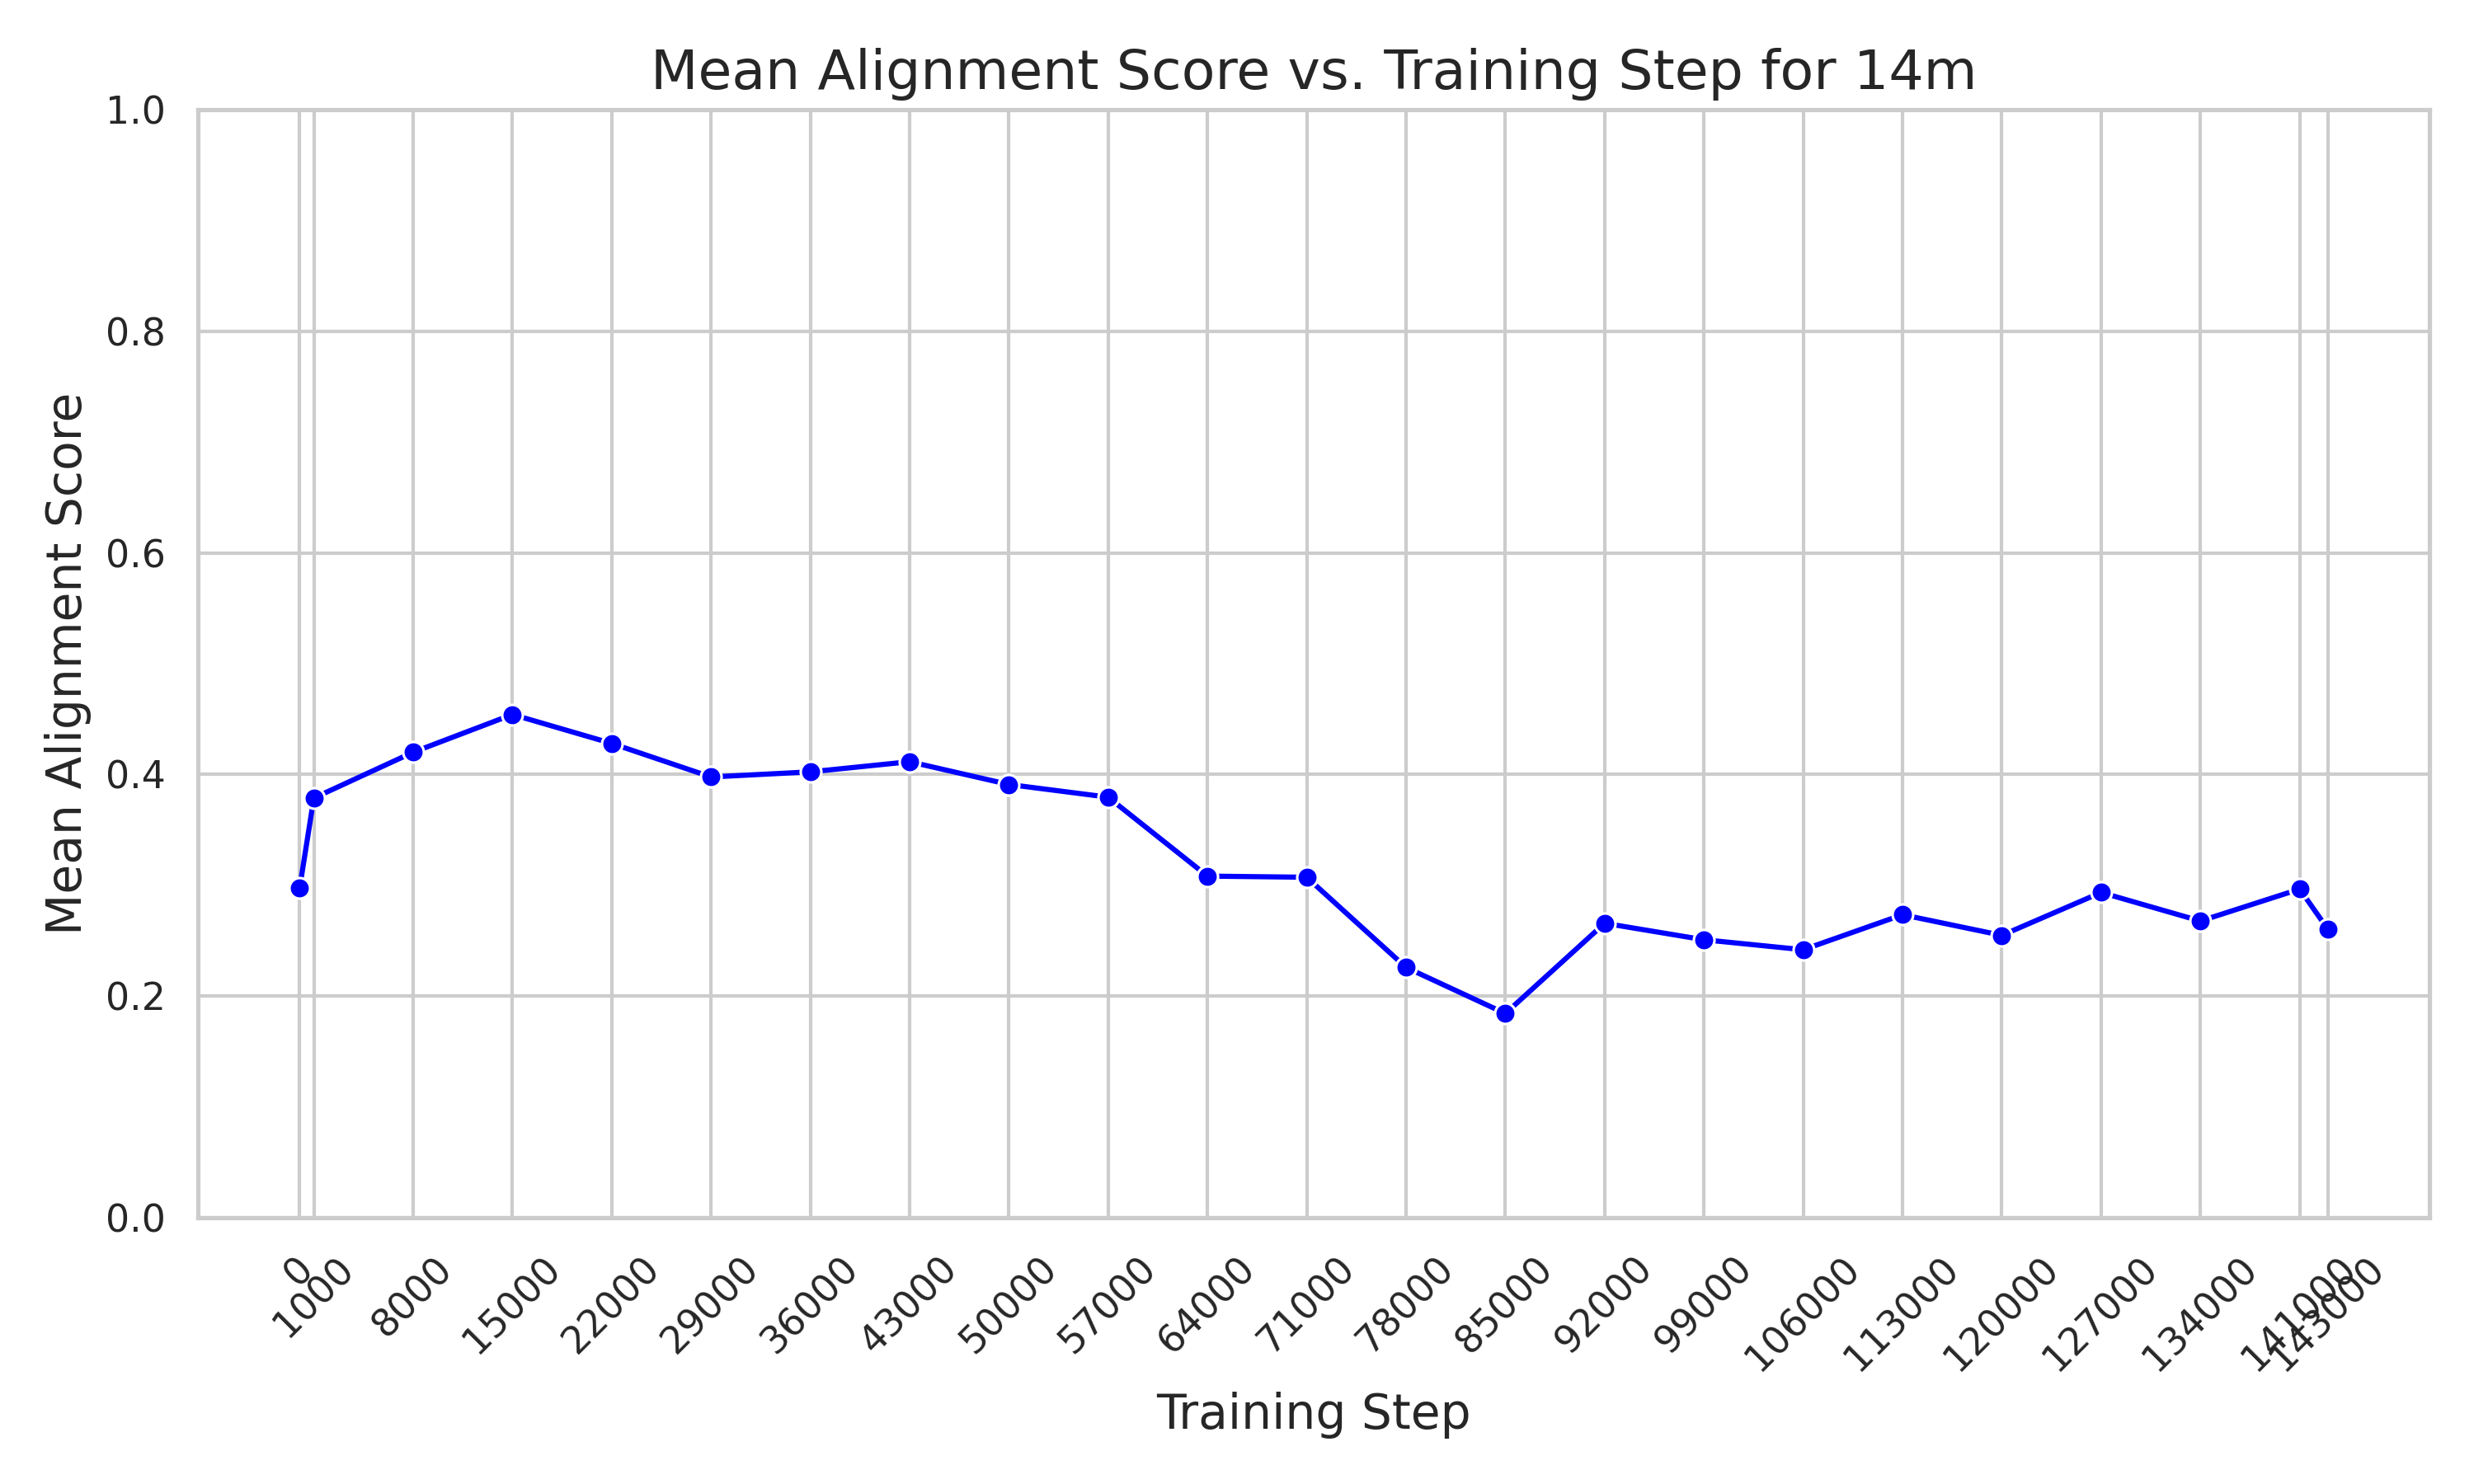
\includegraphics[width=0.48\textwidth]{mean_alignment_score_14m.png}
    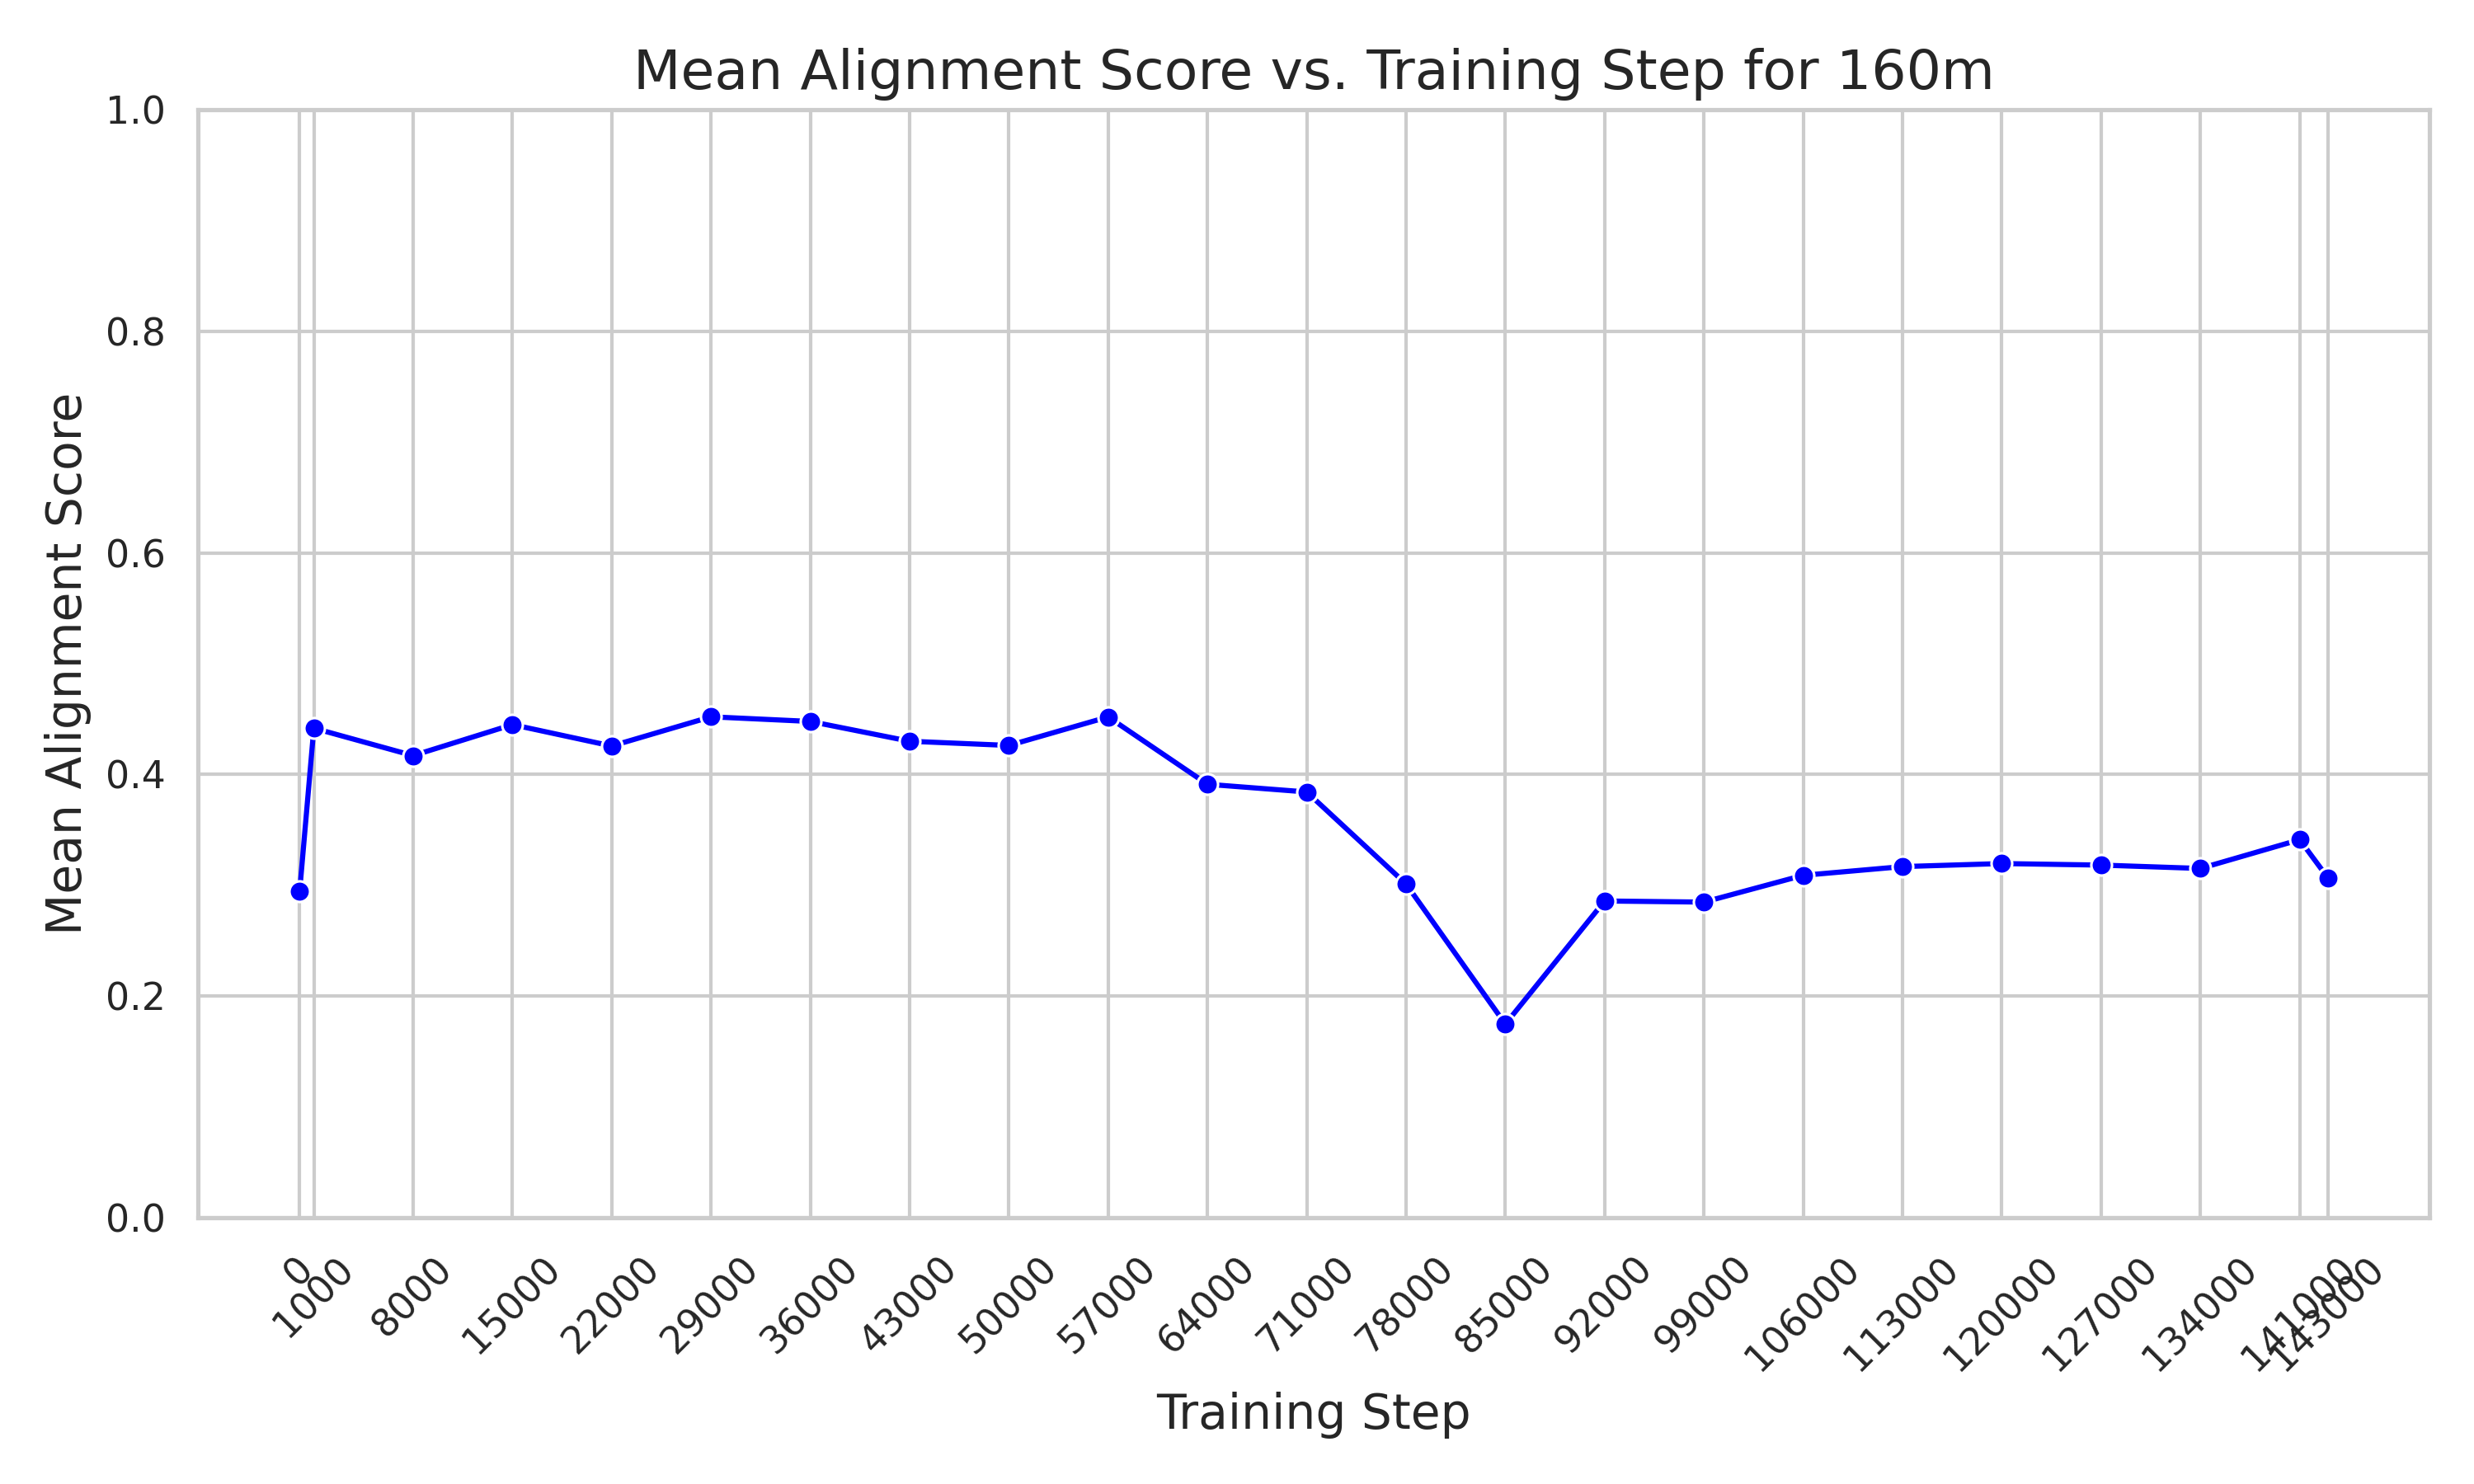
\includegraphics[width=0.48\textwidth]{mean_alignment_score_160m.png}
    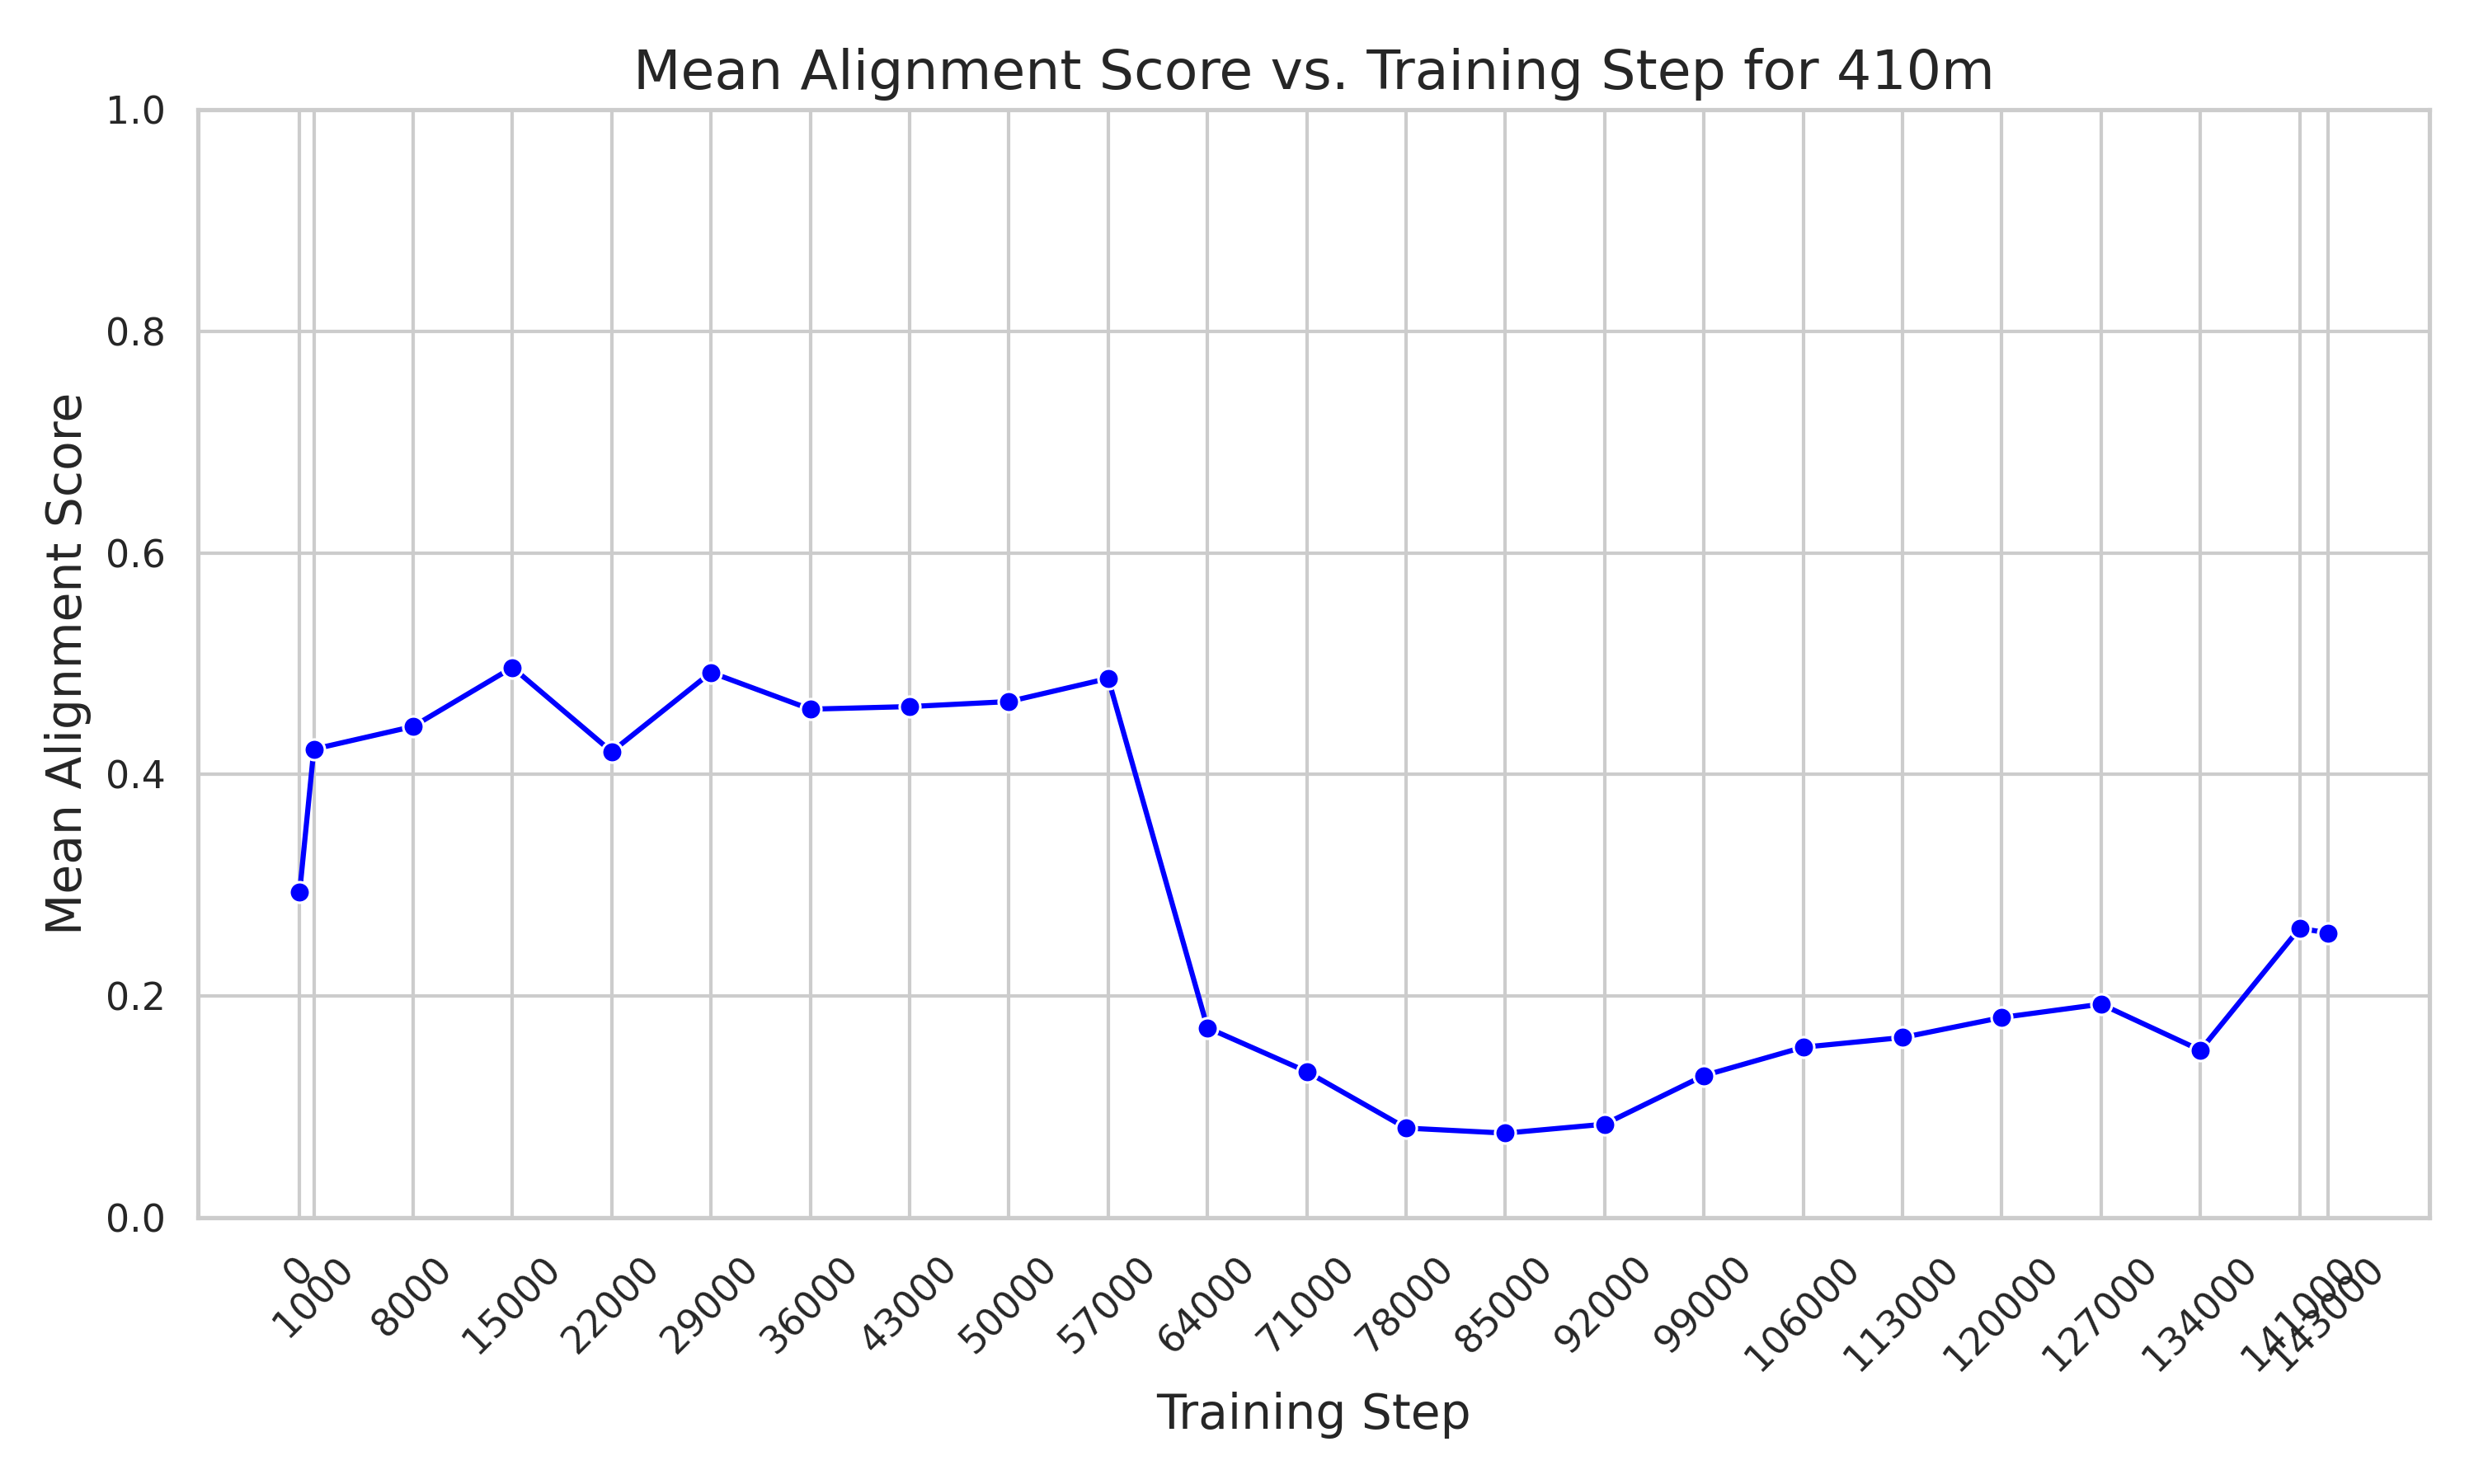
\includegraphics[width=0.48\textwidth]{mean_alignment_score_410m.png}
    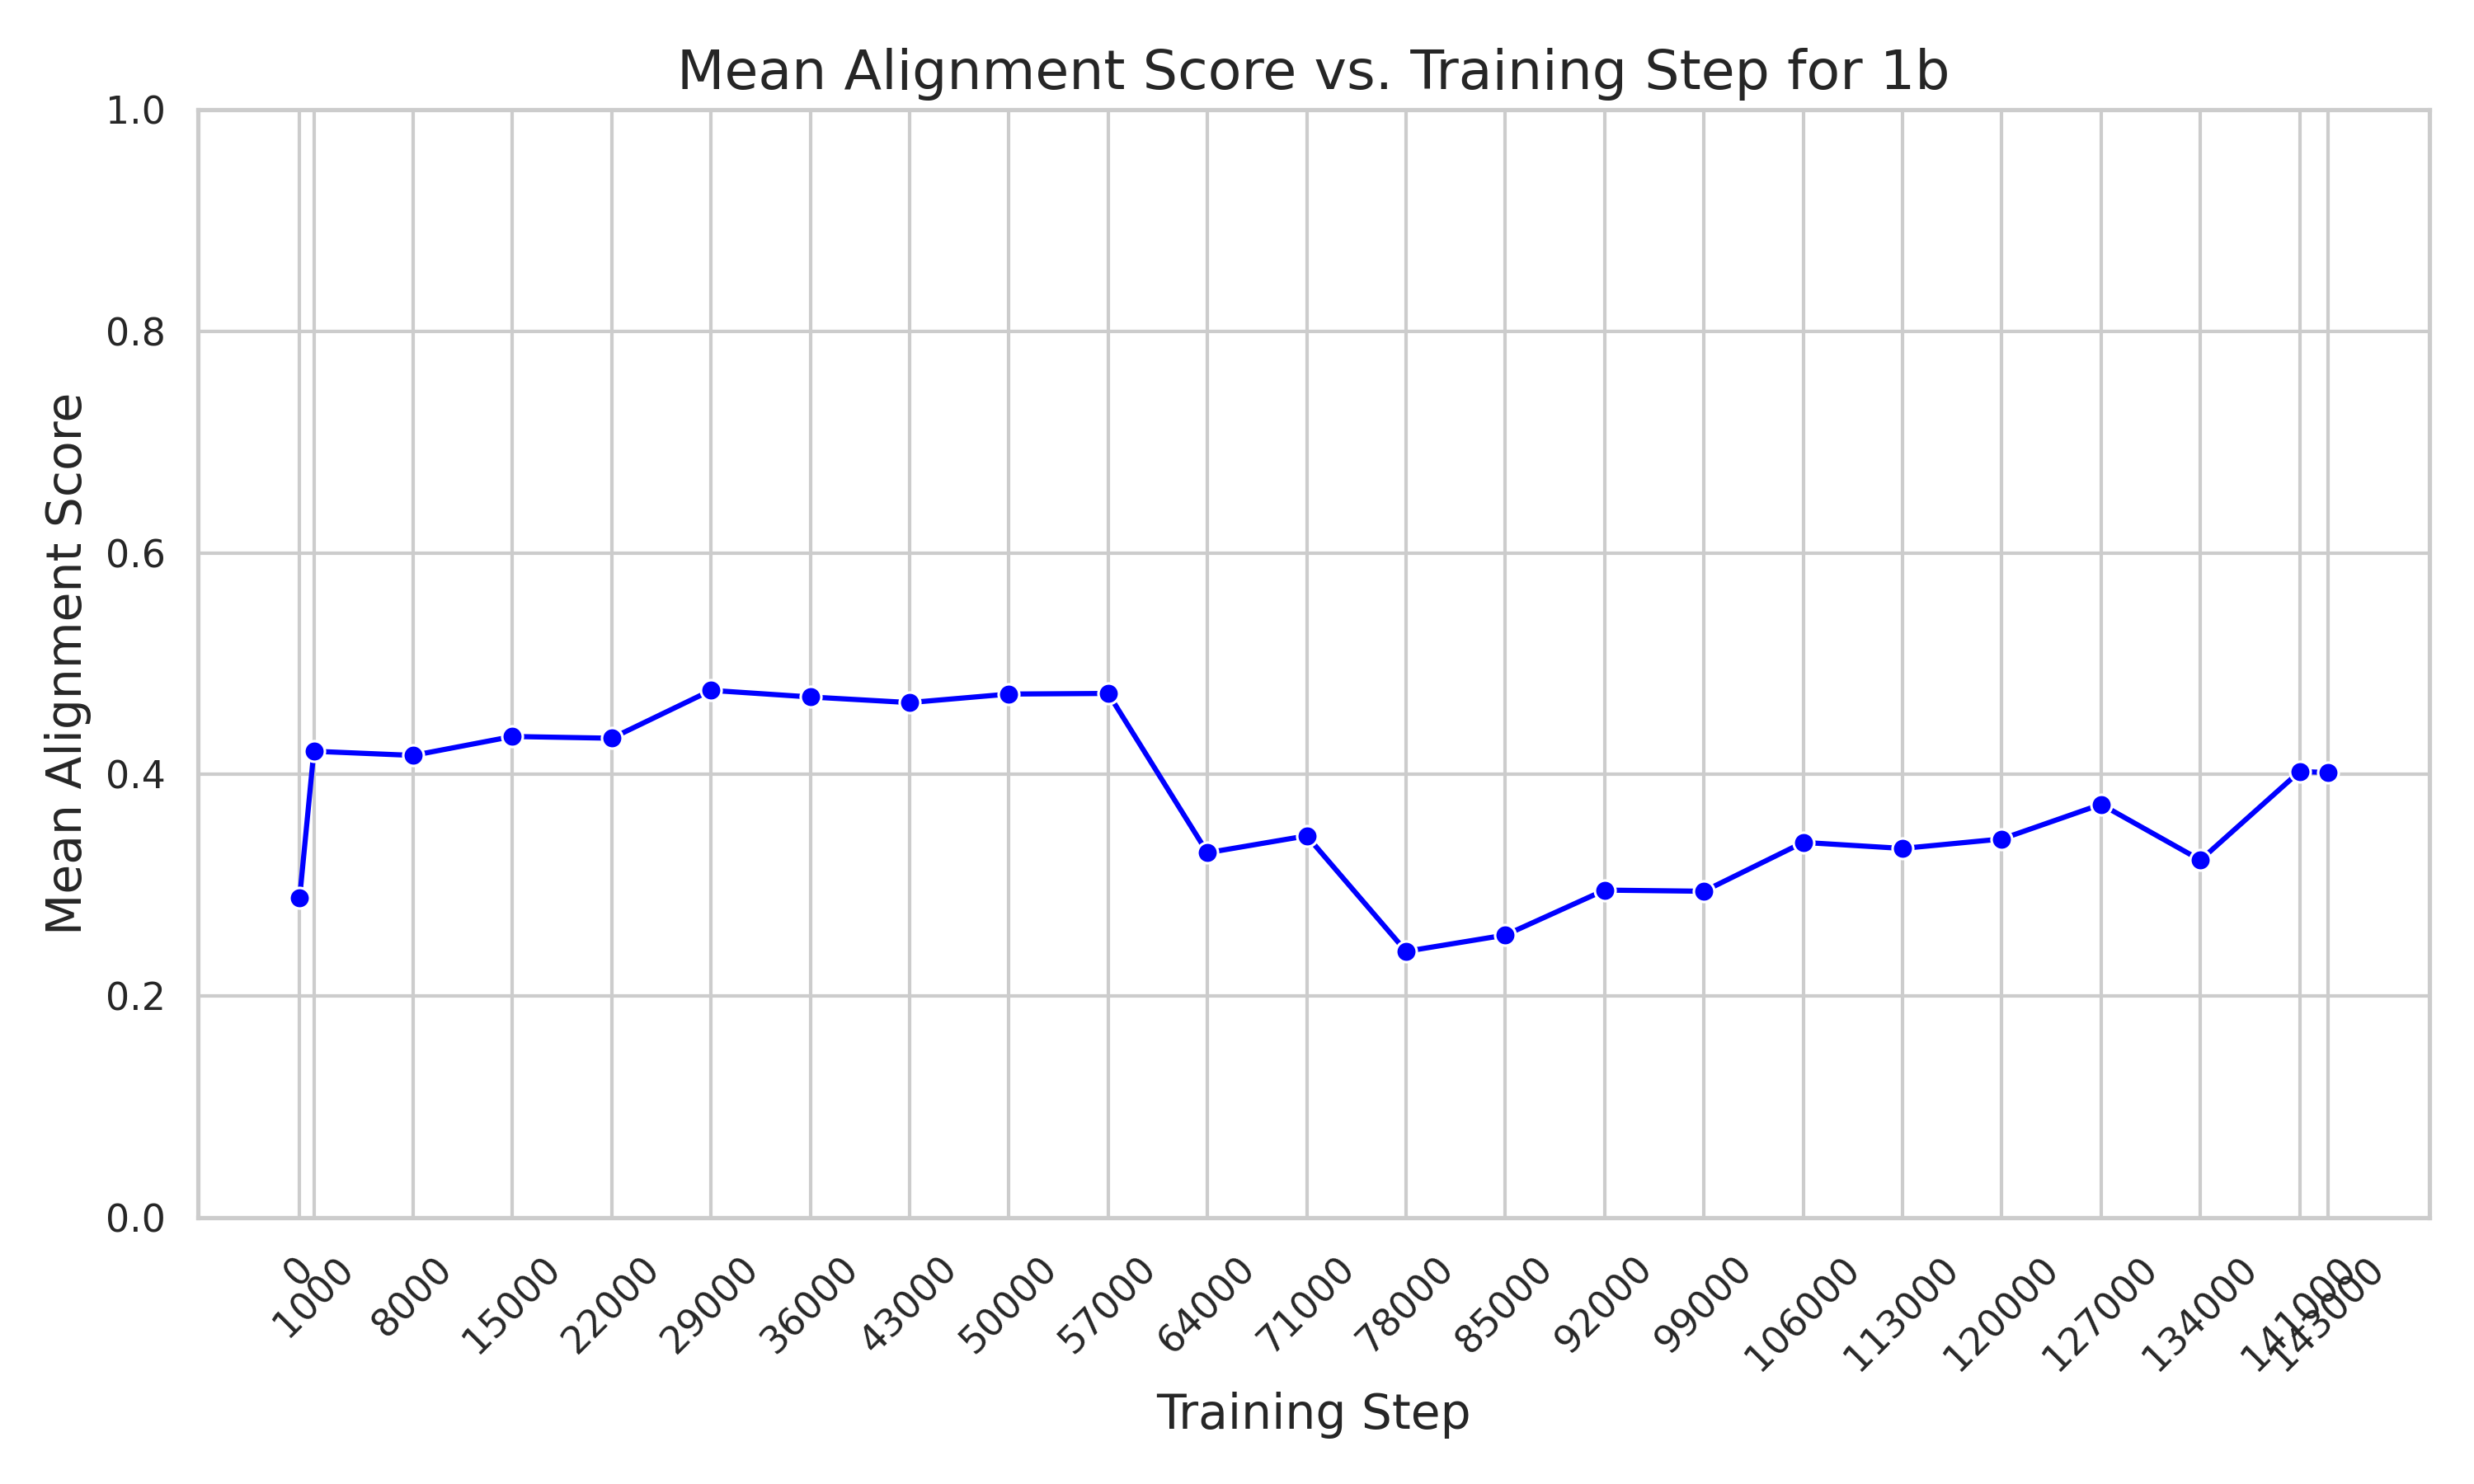
\includegraphics[width=0.48\textwidth]{mean_alignment_score_1b.png}
    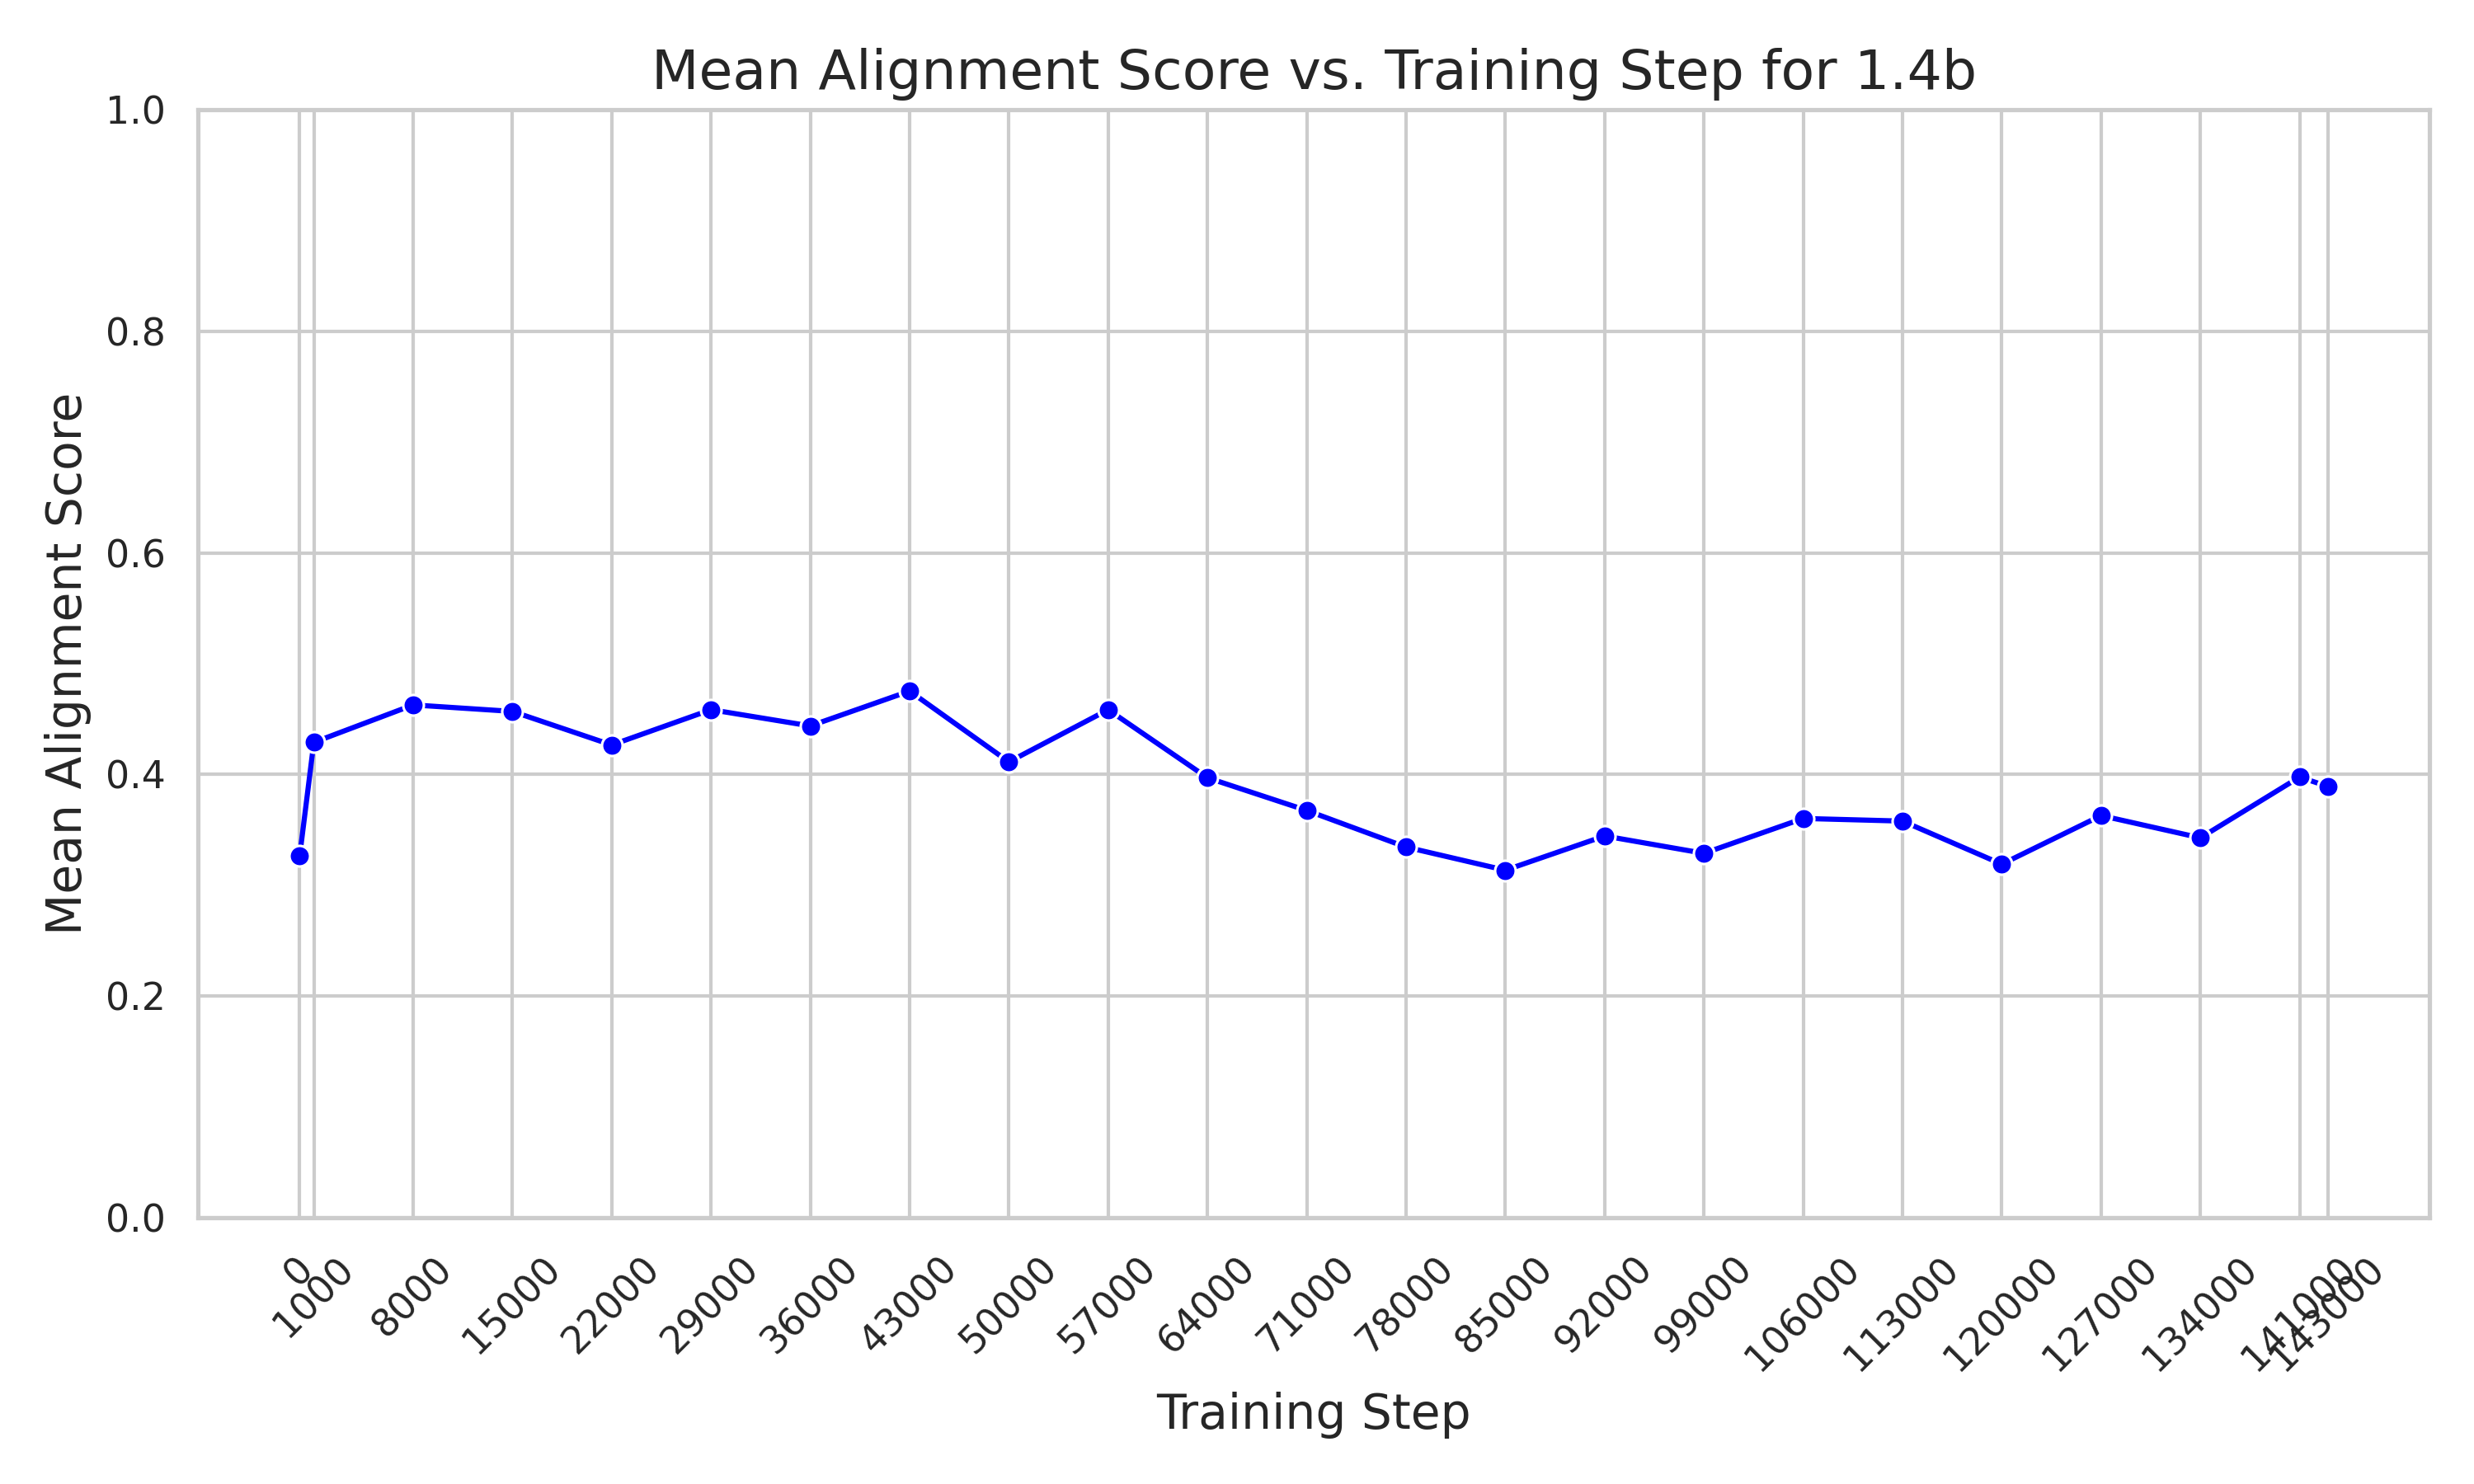
\includegraphics[width=0.48\textwidth]{mean_alignment_score_1.4b.png}
    \caption{Mean alignment scores of language models during training, grouped by the 14M, 160M, 410M, 1B, and 1.4B parameter-sized models. The alignment pattern shows a non-linear trend, characterized by an initial increase, followed by a decline, and then an increase again.}
    \label{fig:llm_training_alignment}
\end{figure}

\section{Discussion}
Our findings show that PRH extends beyond in-distribution data to OOD settings, where models exhibit alignment in their internal representations. On ImageNet-O, models align even in their predictions even when they produce incorrect results with high confidence, revealing that models fail in a predictable manner on OOD data. This suggests that they rely on a shared interpretation of the input space, even when the data diverges from what they have seen during training.

The analysis of noise injection reveals a quadratic relationship between noise levels and representational alignment, suggesting that as noise degrades the input, models align in a predictable manner. This highlights the robustness of model representations to noise, but also their tendency to converge on structured patterns within the data.

The language model training analysis showed a non-linear alignment pattern, which suggests that representational dynamics during training might involve shifts between phases of increased and decreased similarity. This behavior may indicate transitions in how models internalize and abstract from the data.

\section{Conclusion}
The results validate the Platonic Representation Hypothesis in OOD scenarios but highlight its limitations with random noise. Our analysis underscores the need for structured data in achieving representational alignment and suggests new directions for exploring the boundaries of PRH. Future work could focus on extending PRH to other modalities, exploring the effect of different regularization strategies on alignment, and investigating the phases of alignment during language model training.

\vfill
The code used for the experiments and analysis in this paper is available on GitHub \href{https://github.com/rokosbasilisk/prh-experiments}{here}.

\clearpage
\begin{thebibliography}{9}

\bibitem{huh2024prh}
Huh, M., Cheung, B., Wang, T., \& Isola, P. (2024). The Platonic Representation Hypothesis. \emph{International Conference on Machine Learning}.

\bibitem{hendrycks2021nae}
Hendrycks, D., Zhao, K., Basart, S., Steinhardt, J., \& Song, D. (2021). Natural Adversarial Examples. \emph{CVPR}. \href{https://arxiv.org/abs/2405.07987}{arXiv:2405.07987}.

\end{thebibliography}

\end{document}

